Rod-driven continuum parallel robots (RDCPR) represent a relatively novel class of robots characterized by their distinctive rod-driven actuation mechanism. It is of paramount importance to define and limit the dimensions and structural characteristics of these robots, in order to facilitate the development of a platform which will enable the robots to be moved and operated in a variety of applications. The following sections will conduct a detailed exploration of the configuration and essential components that define the structure and operational capabilities of the RDCPR.

\section{Reference Model}

The reference model, depicted in Figure \ref{fig:ref-robot}, was developed by Wu and Shi \cite{wu2022}. The design was selected for its comprehensive representation of an RDCPR, showcasing versatility and a wide range of motion. The robot features two independently manipulable segments, allowing for a total of five degrees of freedom (DoFs), which makes it extensible.

\begin{figure}[H]
    \centering
    \begin{subfigure}[t]{0.3\textwidth}
        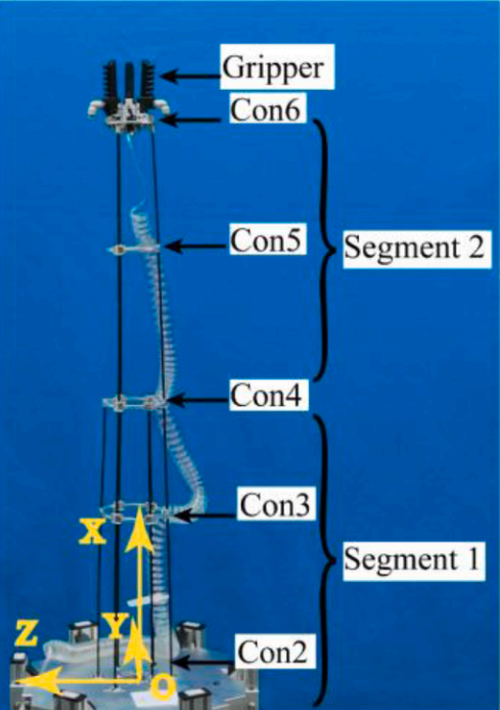
\includegraphics[width=\textwidth]{ref-robot}
        \caption{Sections and structure}
        \label{fig:ref-robot-structure}
    \end{subfigure}
    \begin{subfigure}[t]{0.3\textwidth}
        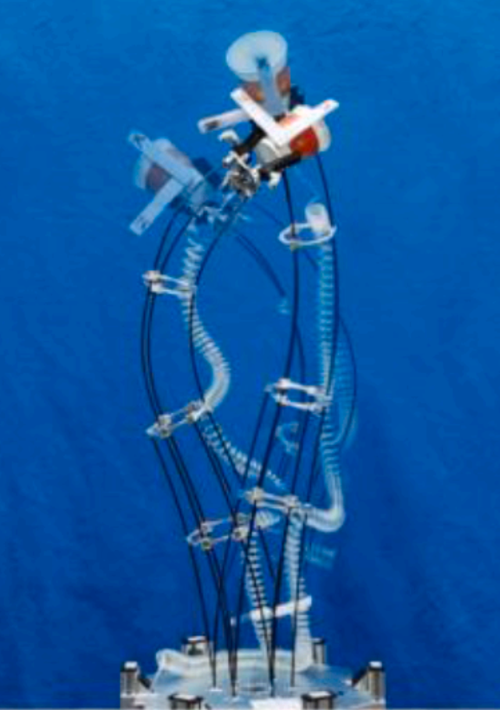
\includegraphics[width=\textwidth]{ref-robot-poses}
        \caption{Some end poses}
        \label{fig:ref-robot-poses}
    \end{subfigure}
    \caption{Reference robot structure}
    \caption*{Source: Adapted from \cite{wu2022}}
    \label{fig:ref-robot}
\end{figure}

The incorporation of intermediate constraints, as Figure \ref{fig:ref-robot2-constraints} illustrates, expands the operational range of the robot.

\begin{figure}[H]
    \centering
    \begin{subfigure}[t]{0.257\textwidth}
        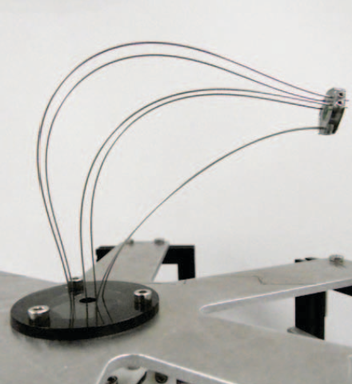
\includegraphics[width=\textwidth]{ref-robot2}
        \caption{No constraints}
        \label{fig:ref-robot2}
    \end{subfigure}
    \begin{subfigure}[t]{0.643\textwidth}
        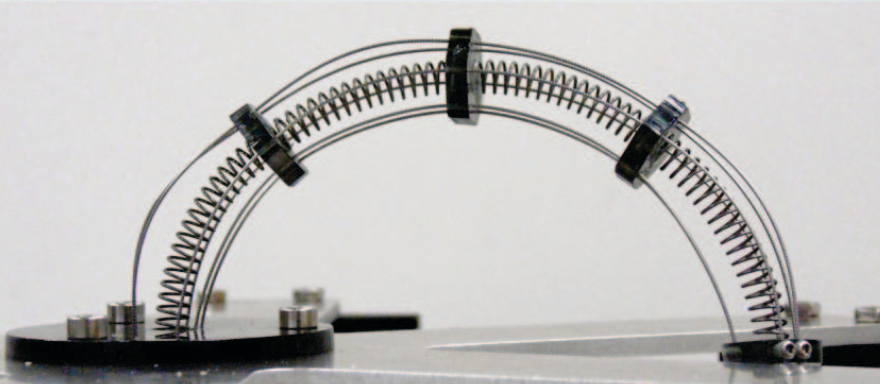
\includegraphics[width=\textwidth]{ref-robot2-cons}
        \caption{Extended range with intermediate constraints}
        \label{fig:ref-robot2-cons}
    \end{subfigure}
    \caption{Constraints and range of motion}
    \caption*{Source: Adapted from \cite{orekhov2017}}
    \label{fig:ref-robot2-constraints}
\end{figure}

\section{Rod Material}

A rod is defined by the inequality \( L \gg r \), where \( L \) represents its length and \( r \) its radius. In the reference model, rods are constructed from fiberglass, whereas in Figure \ref{fig:ref-robot2-constraints}, they are made from steel. These materials are commonly utilized due to their high stiffness and capacity to withstand significant bending without plastic deformation or fracture. Steel alloys, such as AISI 302, which are commonly employed in springs, exemplify these properties. Table \ref{tab:material-properties} provides the material properties of AISI 302 steel and fiberglass.

\begin{table}[h]
    \centering
    \caption{Fiberglass and AISI 302 steel properties}
    \label{tab:material-properties}
    \begin{tabular}{clcc}
    \toprule
    Symbol & Property                   & Fiberglass & AISI 302 \\ \midrule
    $\rho$ & Density [$g/cm^3$]        & 2.6        & 8.0      \\
    $E$    & Young's Modulus [GPa]  & 85         & 187.5    \\
    $G$    & Shearing Modulus [GPa] & 36         & 70.3     \\ \bottomrule
    \end{tabular}
\end{table}


While the Cosserat rod model \cite{russo2023} is commonly used for analyzing these robots, understanding the maximum deflection that a rod can withstand can be determined by applying the Euler-Bernoulli beam equation \ref{eq:max-d}, where \( I \) is given by equation \ref{eq:I}. For the purposes of practicality, a configuration of AISI 302 steel rods was selected due to their commercial availability, with dimensions specified in Table \ref{tab:comparison}. It should be noted that these rods are commonly sold in the form of wire, therefore they had to be straightened prior to use.

\begin{equation}
    \label{eq:max-d}
    \delta_{max}=\frac{PL^3}{3EI}
\end{equation}
\begin{equation}
    \label{eq:I}
    I=\frac{\pi D^4}{64}
\end{equation}

\begin{table}[h]
    \centering
    \caption{Comparison between Wu \& Shi (2022) model and custom test model}
    \label{tab:comparison}
    \begin{tabular}{lcc}
    \toprule
    Parameter                  & \multicolumn{1}{l}{Wu \& Shi model \cite{wu2022}} & \multicolumn{1}{l}{Custom test model} \\ \midrule
    Maximum length             & $\sim860$ mm                     & $\sim450$ mm                       \\
    Minimum length             & $\sim400$ mm                     & $\sim250$ mm                        \\
    Diameters of constraints   & $[90, 80, 70, 60]$ mm               & $[55, 50, 45]$ mm                     \\
    Base constraint diameter   & 100 mm                              & 70 mm                                 \\
    Number of sections         & $2$                                 & $2$                                   \\
    Number of rods             & $6$                                 & $6$                                   \\
    Rod cross-section diameter & $3$ mm                              & $0.8$ mm                              \\
    Rod material               & Fiberglass                          & AISI 302                              \\ \bottomrule
    \end{tabular}
\end{table}

Despite the higher Young's modulus of steel and the necessity for shorter rods with significantly smaller radii, we achieved greater deflections under the same load compared to the reference model. As shown in Figure \ref{fig:force-deflection}, this implies that the same deflection can be achieved with less force, which is advantageous for actuators with limited force capabilities.

\begin{figure}
    \centering
    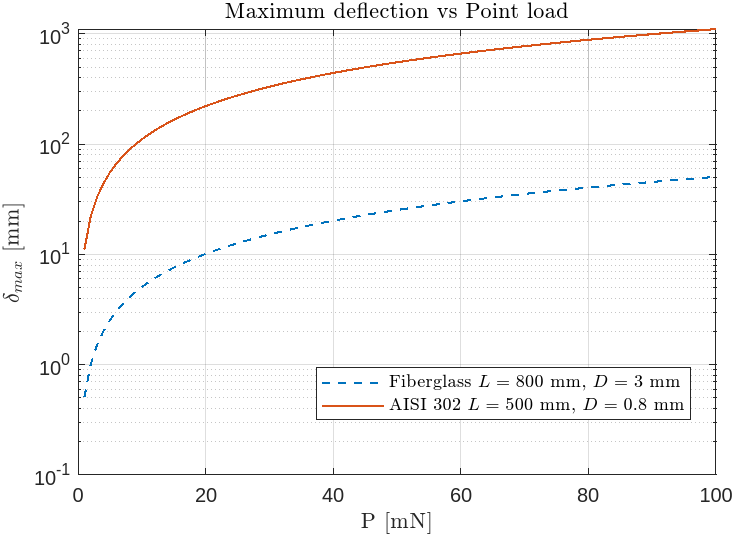
\includegraphics[width=0.8\textwidth]{force-deflection}
    \caption{Maximum deflection and point load}
    \label{fig:force-deflection}
\end{figure}

\section{Design and Dimensions}

To discuss the design and dimensions of the robot's body, the various components are depicted in Figure \ref{fig:bodyparts}. These include rods for the first and second segments, constraints, and joints between constraints and rods. The joints can be either closed-form or cylindrical-form pairs designed to restrict movement. Each intermediate segment is required to have at least one closed-form pair joint with a rod for structural stability, while the remaining joints should be cylindrical to facilitate bending of the arm. At the end of each segment, all joints within the constraints must be closed-form to prevent disassembly of the segment. A minimum of three rods per segment is necessary to maintain structural integrity.

\begin{figure}
    \centering
    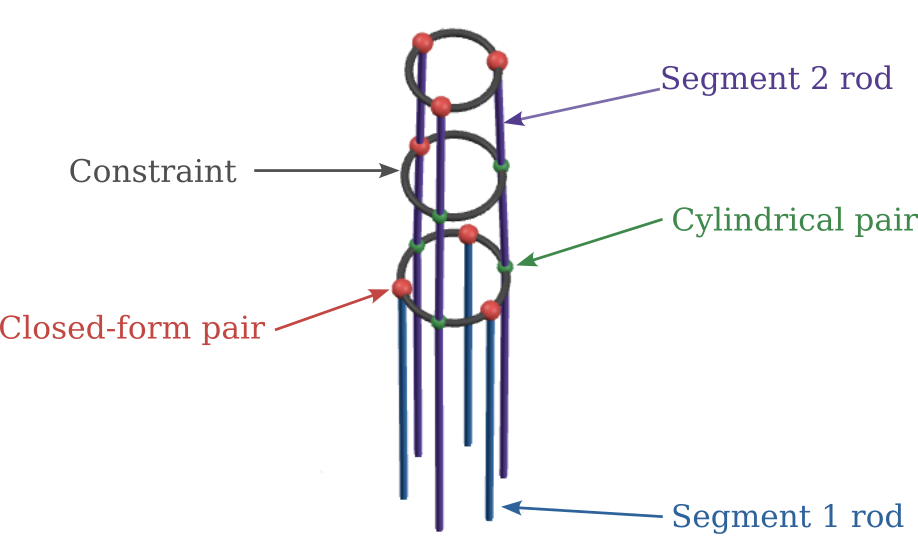
\includegraphics[width=0.6\textwidth]{rod-body-parts}
    \caption{Robot body constraints and parts}
    \label{fig:bodyparts}
\end{figure}

Figure \ref{fig:robot-body-lateral} illustrates the height of each segment and their respective constraints are illustrated. Additionally, the arm exhibits a tapered envelope similar to the reference model. This design choice, influenced by Wu and Shi \cite{wu2022}, enhances structural stiffness. The tapered shape, resembling a truncated cone, is achieved by gradually reducing the cross-sectional area along the length of the arm.

\begin{figure}[H]
    \centering
    \begin{subfigure}[t]{0.2362\textwidth}
        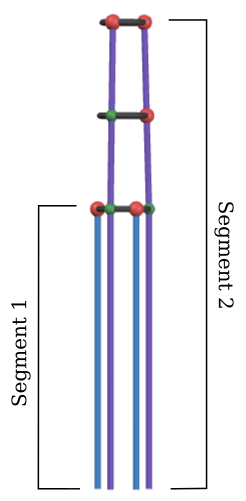
\includegraphics[width=\textwidth]{rod-body-segments}
        \caption{Left view, and robot body segments}
        \label{fig:segments}
    \end{subfigure}
    \begin{subfigure}[t]{0.3937\textwidth}
        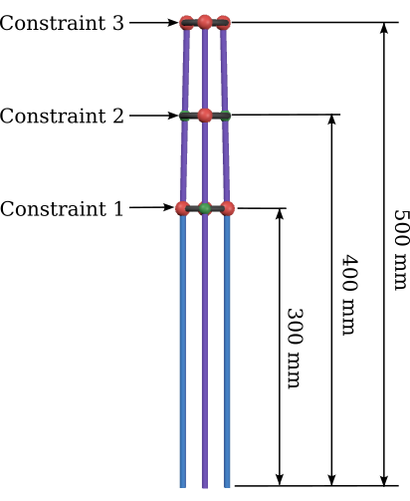
\includegraphics[width=\textwidth]{constraint-heights}
        \caption{Frontal view, and constraints heights}
        \label{fig:cons-heights}
    \end{subfigure}
    \caption{Robot body lateral views}
    \label{fig:robot-body-lateral}
\end{figure}

\section{Ring Constraints}

The proposed constraint design, depicted in Figure \ref{fig:ring-constraint}, takes the form of a ring or hoop and is specifically tailored for additive manufacturing. The shape of the cross-section is of great importance, since it allows for enhancement of the lateral load-bearing capabilities, which in turn mitigate deformation under load. In contrast to traditional rectangular profiles, which are prone to deformation intro ellipses, the selected rhomboidal cross-section provides structural stability. This geometric configuration, which resembles a hollowed-out egg-shaped cylinder in its cross-section, offers enhanced resistance to lateral forces, thereby ensuring robust performance in rod-driven continuous parallel robots.

\begin{figure}[H]
    \centering
    \begin{subfigure}[t]{0.6\textwidth}
        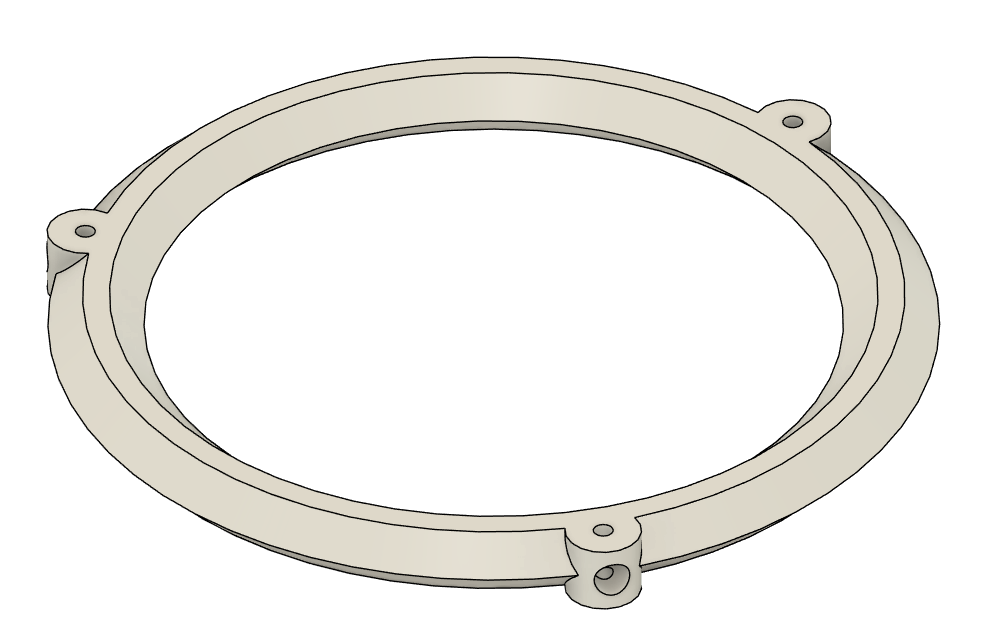
\includegraphics[width=\textwidth]{constraint-view}
        \caption{General view}
        \label{fig:cons-view}
    \end{subfigure}
    \begin{subfigure}[t]{0.6\textwidth}
        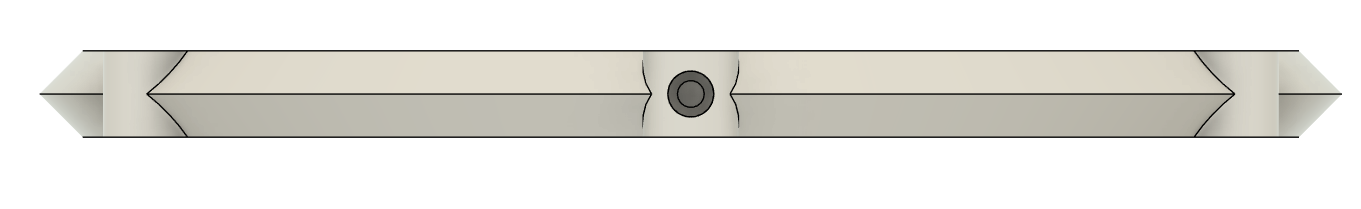
\includegraphics[width=\textwidth]{constraint-frontal-view}
        \caption{Lateral view}
        \label{fig:cons-front-view}
    \end{subfigure}
    \caption{Ring constraint}
    \label{fig:ring-constraint}
\end{figure}

The dimensions of the constraints utilized in the rod-driven continuous parallel robots exhibit variance, as illustrated in Figure \ref{fig:cons-sizes}. These dimensions align with the specifications outlined in Table \ref{tab:comparison}. Each hole of the constraints is tailored to accommodate a specific rod, as indicated by the labels beside the holes. Additionally, the image depicts the type of joint with the constraint, whether closed-form or cylindrical.

\begin{figure}[H]
    \centering
    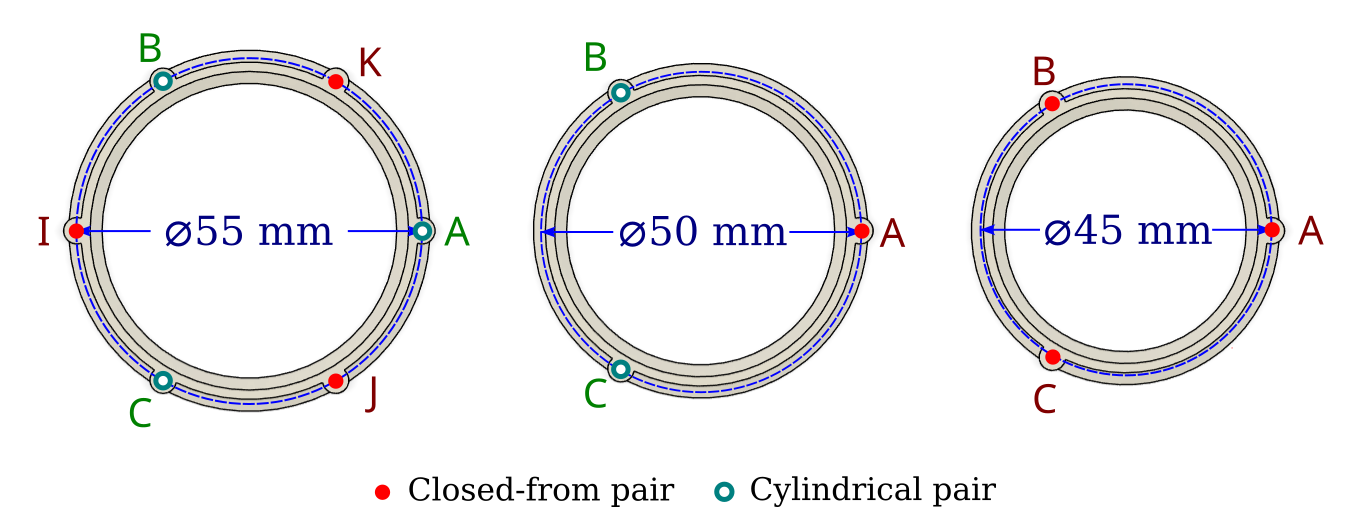
\includegraphics[width=0.9\textwidth]{constraint-sizes}
    \caption{Ring constraint sizes}
    \label{fig:cons-sizes}
    \caption*{In \textit{blue}, the diameters of the circumferences enclosing the rods are shown. The rods are labeled \textit{A}, \textit{B}, \textit{C}, \textit{I}, \textit{J}, \textit{K}. The \textit{green} open circle indicates a cylindrical pair constraint between the ring and the rod, while the \textit{red} indicates a closed-form pair constraint involving both.}
\end{figure}

In terms of physical construction, a closed-form pair joint is created using a set screw that secures the rod in place. This is illustrated in Figure \ref{fig:closed-constraint}. This type of joint provides a firm grip on the rod, preventing any movement. In contrast, a cylindrical-form pair joint is similar in construction but omits the set screw, allowing for both translational and rotational movement along the axis of the hole.

\begin{figure} [H]
    \centering
    \begin{subfigure}[t]{0.45\textwidth}
        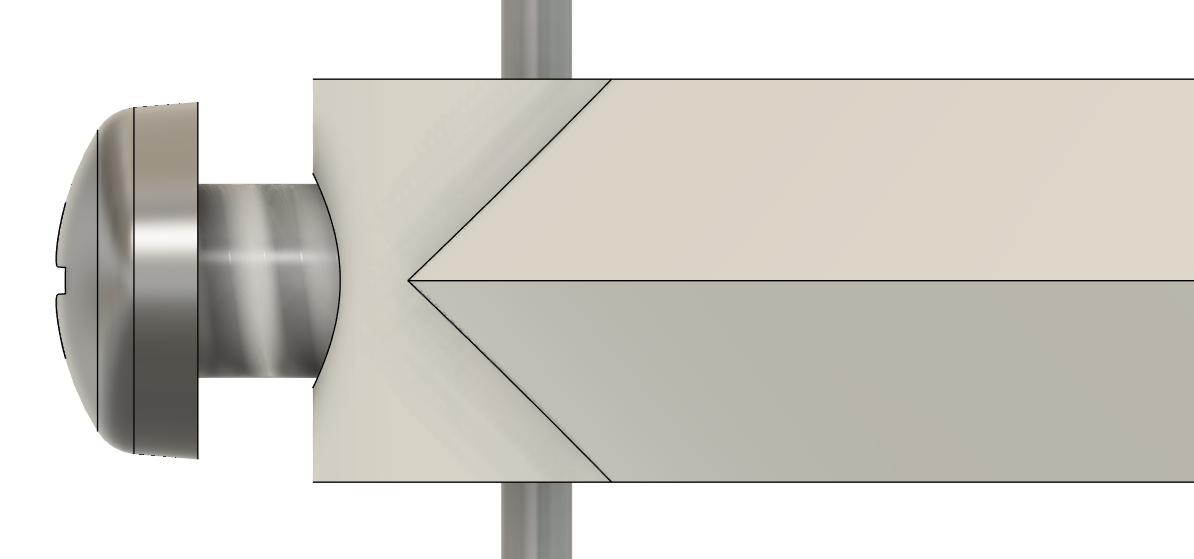
\includegraphics[width=\textwidth]{constraint-screw-rod}
        \caption{Physical closed-form pair constraint}
        \label{fig:cons_physical}
    \end{subfigure}
    \begin{subfigure}[t]{0.45\textwidth}
        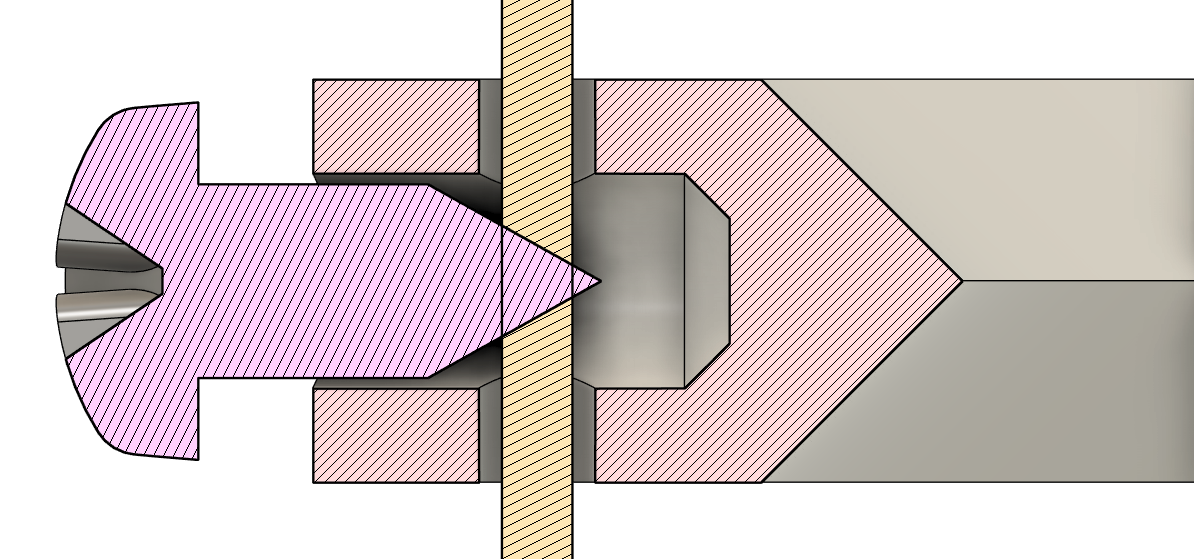
\includegraphics[width=\textwidth]{constraint-section-view}
        \caption{Section view of closed-form pair constraint}
        \label{fig:cons_physical_section}
    \end{subfigure}
    \caption{Closed-form pair constraint}
    \label{fig:closed-constraint}
\end{figure}
